\documentclass[headsepline=true, abstracton]{scrartcl}
%\usepackage[ngerman]{babel}
\usepackage[utf8]{inputenc}
\usepackage[T1]{fontenc}
\usepackage{amssymb}
\usepackage{amsmath}
\usepackage{amsthm}
\usepackage{enumerate}
\usepackage{verbatim}
\usepackage[a4paper,text={140mm,215mm},centering,headsep=10mm,footskip=10mm]{geometry}
\usepackage[urlcolor=black,colorlinks=true,linkcolor=black,citecolor=black,bookmarks]{hyperref}
\usepackage{aliascnt}
\usepackage{lmodern}
\usepackage{mdwlist}
\usepackage{multirow}
\usepackage[table,xcdraw]{xcolor}
\usepackage{listings}
\usepackage[activate]{pdfcprot}
\usepackage{graphicx}
\usepackage{slashed}
\usepackage{mathrsfs}
\usepackage{geometry}
\usepackage{float}
\usepackage{oldgerm}
\usepackage{setspace}
\usepackage{dsfont}
%\usepackage{mathtools}
\usepackage[all]{xy}
\usepackage{cite}
\usepackage{url}
\pagestyle{headings}
\newcommand{\myclearpage}{\clearpage}
\newcommand\independent{\protect\mathpalette{\protect\independenT}{\perp}}
\def\independenT#1#2{\mathrel{\rlap{$#1#2$}\mkern2mu{#1#2}}}
\newenvironment{gelaber}{}{}
\newenvironment{preamble}{}{}
\newcommand{\tostar}{\overset{*}{\lower0.5em\hbox{$\smash{\scriptscriptstyle\rightharpoonup}$}}}
\newtheorem{mydef}{Definition}
\newtheorem{bem}{Bemerkung}
\usepackage{tikz}
\newcommand\circlearound[1]{%
  \tikz[baseline]\node[draw,shape=circle,anchor=base] {#1} ;}
  
\begin{document}

\setcounter{section}{-1}

\renewcommand{\refname}{Bibliography}


\onehalfspacing
\setlength{\headsep}{15mm}


\thispagestyle{plain}

\title{\Large Exponential Random Graph Models with Big Networks: Maximum Pseudolikelihood Estimation and the\\Parametric Bootstrap}
\maketitle

\begin{abstract}
\noindent With the growth of interest in network data across fields, the Exponential Random Graph Model (ERGM) has emerged as the leading approach to the statistical analysis of network data. ERGM parameter estimation requires the approximation of an intractable normalizing constant. Simulation methods represent the state-of-the-art approach to approximating the normalizing constant, leading to estimation by Monte Carlo maximum likelihood (MCMLE). MCMLE is accurate when a large sample of networks is used to approximate the normalizing constant. However, as the size of the network increases, MCMLE is computationally expensive, and may be prohibitively so if the size of the network is on the order of 10,000. When the network is large, one option for estimation is maximum pseudolikelihood (MPLE). MPLE is considerably less accurate than MLE in small networks, but exhibits comparable mean squared error in large networks. The standard MPLE is simple and fast, but generally underestimates standard errors. We show that a resampling method---the parametric bootstrap---results in accurate coverage probabilities for confidence intervals. Furthermore, bootstrapped MPLE has the advantage of being embarrassingly parallel. We compare the two different approaches by applying them on U.S. Supreme Court Citation Network Data.
\end{abstract}


 \section*{Introduction}
 
The field of network science faces a double-edge sword when it comes to computational limitations to innovation. First, the networks under study are growing larger with each year. {\bf [CHRISTIAN, WOULD YOU CHECK OUT N NODES IN {\em SOCIAL NETWORKS}?]}. Second, analytical methods are growing more sophisticated, increasingly involving estimation and optimization, going beyond descriptive calculations {\bf [Could also classify articles based on whether a statistical model is used {\em SOCIAL NETWORKS}?]}. In order to avoid a limiting horizon in which state-of-the-art methods cannot be used with state-of-the-art ``big'' data, network methodologists need to consider all available options in easing the computational burden of tools for network analysis.
 
 \section*{The Exponential Random Graph Model}
The \textit{exponential random graph model} (ERGM) is a probability model for directed or undirected binary networks. This means neither the weighting nor the temporal change of ties is considered in the model.
In literature, ERGMs are sometimes also referred to as \textit{p-star} or $p^*$ models (see Wassermann and Pattison \cite{Wasserman.1996}, Robins et al. \cite{robins.pattison.2007}). In the following, we will focus on directed networks; however, undirected networks can be introduced very similar.\\[0.3cm] 
The ERGM takes the adjacency matrix of an observed network $G^{obs}$ as the manifestation of a matrix-like random variable $Y$. This means that a network of $N$ nodes can be defined as a adjacency matrix $G=(g_{ij})\in \mathbb{R}^{N \times N}$, where $g_{ij} \in \{0,1\}$ for all $i,j \in \{1,\dots , N\}$. $g_{ij}=1$ means that there is an edge between actors $i$ and $j$, while $g_{ij}=0$ indicates that these actors are not directly connected. Since the model does not consider loops, one has $g_{ii}=0$ for all $i \in \{1,\dots , N\}$. Furthermore, define
$$ \mathcal{G}(N) := \left\{ G \in \mathbb{R}^{(N \times N)}: g_{ij} \in \{0,1\},~g_{ii}=0\right\}$$
as the set of all possible networks on $N$ nodes without loops. Note that the cardinality of set $\mathcal{G}(N)$ is increasing exponentially for every newly included actor, which results in $2^{N(N-1)/2}$ total elements. Therefore, for an already small number of actors the cardinality of $\mathcal{G}(N)$ turns out to be an astronomically large number. For this reason calculating the MLE is either extremely time-consuming or with today's technology not achievable. As a consequence, literature usually makes use of Markov Chain Monte Carlo (MCMC) methods.\\  
With the definition of $\mathcal{G}(N)$ we define 
$$Y: \Omega \to \mathcal{G}(N)~~,~~\omega \mapsto (Y_{ij}(\omega))_{i,j=1,\dots,N}$$
as a matrix-like random variable. As the probability function from $Y$ to $\mathcal{G}(N_V)$ we define the ERGM as
\begin{equation}
\mathbb{P}_{\theta}(Y=G)=\dfrac{\exp(\theta^T \cdot \Gamma(G))}{\sum_{G^* \in \mathcal{G}(N)} \exp(\theta^T \cdot \Gamma(G^*))} 
\label{ERGM}
\end{equation}
%
where $\theta \in \mathbb{R}^q$ is a $q-$dimensional vector of parameters, $\Gamma:\mathcal{G}(N) \to \mathbb{R}^q~,~G \mapsto (\Gamma_1(G),\dots,\Gamma_q(G))^T$ is a $q$-dimensional function of different network statistics and $c(\theta):= \sum_{G^* \in \mathcal{G}(N)} \exp(\theta^T \cdot \Gamma(G^*))$ is a normalization constant which ensures that (\ref{ERGM}) defines a probability function on $\mathcal{G}$.
%
As already mentioned, a specific network $G$ can be considered as a manifestation of a matrix-like random variable, whose probability of occurrence can be modeled with equation (\ref{ERGM}).
A key role when modeling an ERGM is played by the function $\Gamma(\cdot)$. The decision about which network statistics are incorporated into the model affects the model significantly (see Handcock \cite{Handcock.2003}).

\section*{Estimation}
As mentioned above calculating $c(\theta)$ is not achievable for most cases with today's technology. Therefore, the question arises how one can estimate the parameter vector $\theta$?
A first idea could be the following: One can assume that the \textit{dyads} are independent of each other, which means that the random variables $Y_{ij}$ inside the random matrix $Y$ are independent of each other. 
In this case, one can show that
%
\begin{equation*}
\text{logit}(\mathbb{P}_{\theta}(Y_{ij}=1))= \theta^T \cdot (\Delta G)_{ij}
%\label{ILogit}
\end{equation*}
This corresponds with the \textit{logistic regression} approach, where the observations of the dependent variables are simply edge values of the observed adjacency matrix, and the observations of the covariate values are given as the scores of every single change statistic. Therefore, the estimation of $\theta$ can then be obtained as usual using straight forward maximum-likelihood estimation. The resulting likelihood function is of the following form:
\begin{equation}
\text{lik}(\theta)= \mathbb{P}_{\theta}(Y=G)= \prod_{i,j} \dfrac{ \exp \left(\theta^T \Delta(G))_{ij} \right)}{1+\exp \left(\theta^T \Delta(G))_{ij} \right)}
\label{NaiveLik}
\end{equation}
The problem with this simple estimation procedure is that the assumed hypothesis of the independence of the dyads turns out to be erroneous in many cases (see van Duijn et al. \cite{vanDuijnetal2009}). This is a systematic problem: The presence of network data is inextricably connected with the presence of \textit{relational data}, which by definition should not be assumed to be independent of each other. If this dependency structure is deliberately ignored and equation (\ref{NaiveLik}) is used to estimate $\theta$, it results in a \textit{maximum pseudo-likelihood estimation} (MPLE). This technique tends to underestimate the standard error. However, Desmarais and Cranmer \cite{Desmarais.2012} show that the pseudo-likelihood provides a consistent approximation of the maximum likelihood, meaning that the MPLE converges to the MLE as the size of the network increases.\\[0.3cm]
There are several techniques to circumvent estimators, which underestimate the standard error of $\theta$. In the following, we will introduce a technique based on \textit{Markov Chain Monte Carlo (MCMC)} and maximum-likelihood methods.\\[0.3cm]
The more rigorous technique is to estimate the parameters directly with the log-likelihood function derived from (\ref{ERGM}), which has the following form:
%
\begin{equation}
\text{loglik}(\theta)=\theta^T \cdot \Gamma(G)-\log(c(\theta))
\label{loglik}
\end{equation}
%
where $G$ is the observed network. For the vector of network statistics, one can assume without loss of generality
%
\begin{equation}
\Gamma(G)=0 \label{assumption}
\end{equation}
%
This means that centering the vector of network statistics does not affect the probability function of the network variable $Y$. Therefore, in context of the likelihood function (\ref{loglik}) the vector of statistics can always be assumed to be centered on the observed network.\\
Due to assumption (\ref{assumption}), one gets from (\ref{loglik}) the simplified log-likelihood function
%
\begin{equation}
\text{loglik}(\theta)= -\log(c(\theta))
\label{vloglik}
\end{equation}
%
The problem resulting from estimating the parameters with (\ref{loglik}) is that the term
%
$$c(\theta):= \sum_{G^* \in \mathcal{G}(N_V)} \exp(\theta^T \cdot \Gamma(G^*))$$ 
%
which sums up the weighted network statistics of all possible networks of $N$ nodes, has to be evaluated. Even for networks with small numbers of nodes this presents an enormous computational obstacle, and the necessary calculations for larger networks cannot currently be completed in any reasonable timeframe.
As a result, for sufficiently large networks it is not possible to estimate the parameters directly with the likelihood function.
\\[0.3cm]
An expedient for this limitation is based on the following consideration: Fix any vector of parameters $\theta_0 \in \Theta$ from the underlying parameter range $\Theta$ and compute for $\theta \in \Theta$ the expected value. Then, one can show that
%
\begin{equation*}
\mathbb{E}_{\theta_0}\left[ \exp\left((\theta - \theta_0)^T \cdot \Gamma(Y)\right) \right]=\frac{c(\theta)}{c(\theta_0)}
\end{equation*}
%
This equation offers the following possibility: If one draws $L$ random networks $G_1, \dots ,G_L$ out of a distribution $\mathbb{P}_{\theta_0}$ appropriately, one gets with the \textit{law of big numbers} the following relation:
%
\begin{equation}
\frac{1}{L}\cdot \sum_{i=1}^{L}  \exp\left((\theta - \theta_0)^T \cdot \Gamma(G_i)\right)
~~\stackrel {{\tiny\mathbb{P}_{\theta_0}}}{\longrightarrow}~~ \mathbb{E}_{\theta_0}\left[ \exp\left((\theta - \theta_0)^T \cdot \Gamma(Y)\right) \right] = \frac{c(\theta)}{c(\theta_0)}
\label{konver}
\end{equation}
%
For a big enough number, $L$, of random networks, the following approximation is reasonable:
%
\begin{equation}
\frac{c(\theta)}{c(\theta_0)} \approx \frac{1}{L}\cdot \sum_{i=1}^{L}  \exp\left((\theta - \theta_0)^T \cdot \Gamma(G_i)\right)
\label{approx}
\end{equation}
%
One can now use equation (\ref{approx}) to determine an approximation of the log-likelihood function (\ref{vloglik}):
%
\begin{eqnarray*}
\text{loglik}(\theta)-\text{loglik}(\theta_0)&=&- \log(c(\theta))+\log(c(\theta_0))\\
                                             &=&- \log \left( \frac{c(\theta)}{c(\theta_0)} \right)\\
                                             &=&- \log \left( \mathbb{E}_{\theta_0}\left[ \exp\left((\theta - \theta_0)^T \cdot \Gamma(Y)\right) \right] \right)\\
                                             &\approx &- \log \left( \frac{1}{L} \cdot \sum_{i=1}^{L}  \exp \left((\theta - \theta_0)^T \cdot \Gamma(G_i) \right) \right)
\end{eqnarray*}
%
By differentiating this equation on both sides with respect to $\theta$ one gets an approximate score function:
%
\begin{equation}
s(\theta) \approx -\frac{\partial}{\partial \theta} \log \left( \frac{1}{L} \cdot \sum_{i=1}^{L}  \exp \left((\theta - \theta_0)^T \cdot \Gamma(G_i) \right) \right)
\label{score}
\end{equation}
%
This approximate score function now can be used as usual, i.e., it can be iteratively approximately optimized with the \textit{Newton-Raphson algorithm}. As a result, the approximate maximum-likelihood estimator for the parameters can be computed.\\[0.4cm]
As pleasant as this may sound, the immediate question arises: How can a sufficient number of suitable drawings $G_1,...,G_L$ be taken from the distribution $\mathbb{P}_{\theta_0}$? \\
For this purpose, the \textit{Markov Chain Monte Carlo (MCMC)} methods can be used. This approach does not deliberately ignore the dependency structures inside the network. Furthermore, the Markov Chain Monte Carlo Maximum Likelihood Estimator (MCMLE) approaches the MLE as the number of networks simulated to approximate the likelihood goes to infinity.\\[0.3cm]

No matter which kind of MCMC algorithm is used, the basic idea is the following:
\\One constructs a \textit{Markov chain} $(Y_t)_{t \in \mathbb{N}}$ on the set of all possible networks $\mathcal{A}(N)$ of $N$ nodes, whose \textit{stationary distribution} is in conformity with the distribution $\mathbb{P}_{\theta_0}$. One can show that every single realization (or \textit{trajectory}) 
of this stochastic process accomplishes the convergence result (\ref{konver}) (for this version of the \textit{Law of big numbers for Markov chains} we reference Meyn and Tweedie \cite{Meyn.2009}). As a result, sub-sequences of $(A_t)_{t \in \mathbb{N}}$ which are sufficiently large enough can be used for approximation (\ref{approx}).\\[0.3cm]
Snijders \cite{Snijders.2002} provides a Metropolis Hastings algorithm on how to simulate networks:
Choose a matrix $G^{(0)} \in \mathcal{G}(N)$ to start with (e.g., the observed network). For $k \in \{0,...,L-1\}$ recursively proceed as follows:\\
\begin{enumerate}
\item Randomly choose an edge $(i,j)$ where $i \neq j$ from $G^{(k)}$
\item Compute the value
$$\pi := \dfrac{\mathbb{P}_{\theta}(Y_{ij} \neq g_{ij}^{(k)} | Y_{ij}^c=G_{ij}^c)}{\mathbb{P}_{\theta}(Y_{ij}= g_{ij}^{(k)} | Y_{ij}^c=G_{ij}^c)}$$
\item Fix $\delta:= \min\{1, \pi\}$ and draw a random number $Z$ from Bin$(1, \delta)$. If
\begin{itemize}
\item $Z=0$, let $G^{(k+1)} := G^{(k)}$ 
\item $Z=1$, define $G^{(k+1)}$ via
$$g_{pq}^{(k+1)}=\begin{cases}
1-g_{pq}^{(k)}& \text{if}~ (p,q)=(i,j) \\
g_{pq}^{(k)} &\text{if}~ (p,q) \neq (i,j) 
\end{cases}$$
\end{itemize}
\item Start at step 1 with $G^{(k+1)}$.
\end{enumerate}
The depicted algorithm provides a sequence of random networks $G_(0),\dots,G_(L)$. Since the original matrix was chosen randomly and the first simulated networks are very dependent on the chosen matrix (only one edge is changed per iteration), usually
the first $B$ networks, where $N << B << L$, are discarded as the so called Burn-In.




\section*{Efficiency of MPLE/MCMLE}
Even though the MCMLE is in general favored over the MPLE method there are also cases where the MPLE comes in handy. Foremost, MPLE is quick and simple, since estimation can be done by basic logistic regression and does not exert elaborate MCMC methods. As mentioned in the previous chapter the MPLE approaches the MLE as the size of the networks increase and as a consequence, is a consistent estimator (see Lindsay \cite{Lindsay1988}, Strauss and Ikeda \cite{StraussIkeda1990}, Hyvarinen \cite{Hyvarinen2006}, Desmarais and Cranmer \cite{Desmarais.2012}). This implies that for an increasing number of nodes the MPLE converges in probability to the MLE, meaning that for large enough networks the MPLE becomes an option to computationally intensive MCMC methods.\\
At this point we want to mention that we are familiar with the work of Shalizi and Rinaldo \cite{shalizi2013}, arguing that consistency is not given in the ERGM framework. They prove that one cannot run an ERGM on a sub-network in order to make inferences about the full network. 
The way we use the term \textit{consistency} in this paper is different and aligns with the way consistency is seen by Lindsay \cite{Lindsay1988}, i.e. instead of considering sub-networks, we argue that both, the MLE as well as the MPLE, approach the true coefficient values as the size of networks increases. \\%This means that the MPLE of a network on $1000$ nodes is closer to the true coefficient as the MPLE of a network on $100$ nodes. \\
\textcolor{red}{Another major advantage of the MCMLE method is, as shown by van Duijn et al. \cite{vanDuijnetal2009}, that the MCMLE is a more efficient estimator than the MPLE, meaning that the variance of the MCMLE is in general lower than the variance of the MPLE.-Rewrite} Nevertheless, as shown by Desmarais and Cranmer \cite{Desmarais.2012} the MPLE outperforms the MCMLE if the number of simulated networks used to approximate the likelihood is not chosen large enough. It is even more remarkable that the number of simulated networks needed for the MCMLE, in order to surpass the MPLE increases as the size of the network increases. This means that for very large networks it becomes difficult to determine the number of simulated networks needed in order for the MCMLE to outperform the MPLE. In other words, the larger the network of interest is, the larger one has to choose the number of simulated networks in order to justify the time intensive MCMLE approach.\\[0.3cm]
\noindent In order to demonstrate this disadvantage of the MCMLE we conduct a simulation study using Goodreau's Faux Mesa High School data, which represents a simulation of an in-school friendship network among 203 students as well as the Faux Magnolia High School data, representing an in-school friendship network among 1451 students. The data for both networks originates from Resnick et al \cite{Resnicketal1997}.\\[0.3cm]
For both networks we first calculate the MCMLE and treat the estimated coefficients as the network's true values $\theta$. For both networks we take the same parametrization, using the number of edges, the nodal attribute for gender and the geometrically weighted edgewise shared partners (gwesp)(see Hunter \cite{Hunter.2006}) distribution were we fix the decay parameter $\lambda$ at $0.25$.\\
We simulate 500 new networks using the 'true' coefficients and estimate the MPLE as well as the MCMLE of these simulated networks. For every single simulated network the MCMLE calculation is being repeated several times using 1500, 800, 400, 200, 100, 50 and 25 simulated networks in order to approximate the likelihood.
Based on these results, we compute the root mean square error, which is a measure of the accuracy of an estimator, combining both, the bias and the variance. Mathematically written, the RMSE for an estimator $\hat{\theta}$ is defined as 
$$RMSE = \sqrt{\sum_{i=1}^{500}(\theta - \hat{\theta}_i)^2}$$
implying that the smaller the RMSE, the more accurate is the estimator. Since the MCMLE has higher efficiency and converges to the MLE, the RMSE decreases as the number of simulated networks used for the likelihood approximation increases. On the other hand, the RMSE of the MPLE is a constant value since no network simulations are required. In order to compare the RMSE of the two estimation techniques, we take the log of the ratio of the MCMLE to the MPLE. As a result, a negative value indicates a better MCMLE performance, while a positive value indicates a better MPLE performance. Figure \ref{rmse} visualizes the results of the simulation study. The solid line illustrates the results of the log relative RMSE of the Faux Mesa High network, while the dashed line illustrates the corresponding results of the Faux Magnolia High network. 

\begin{figure}[h]
\begin{center}
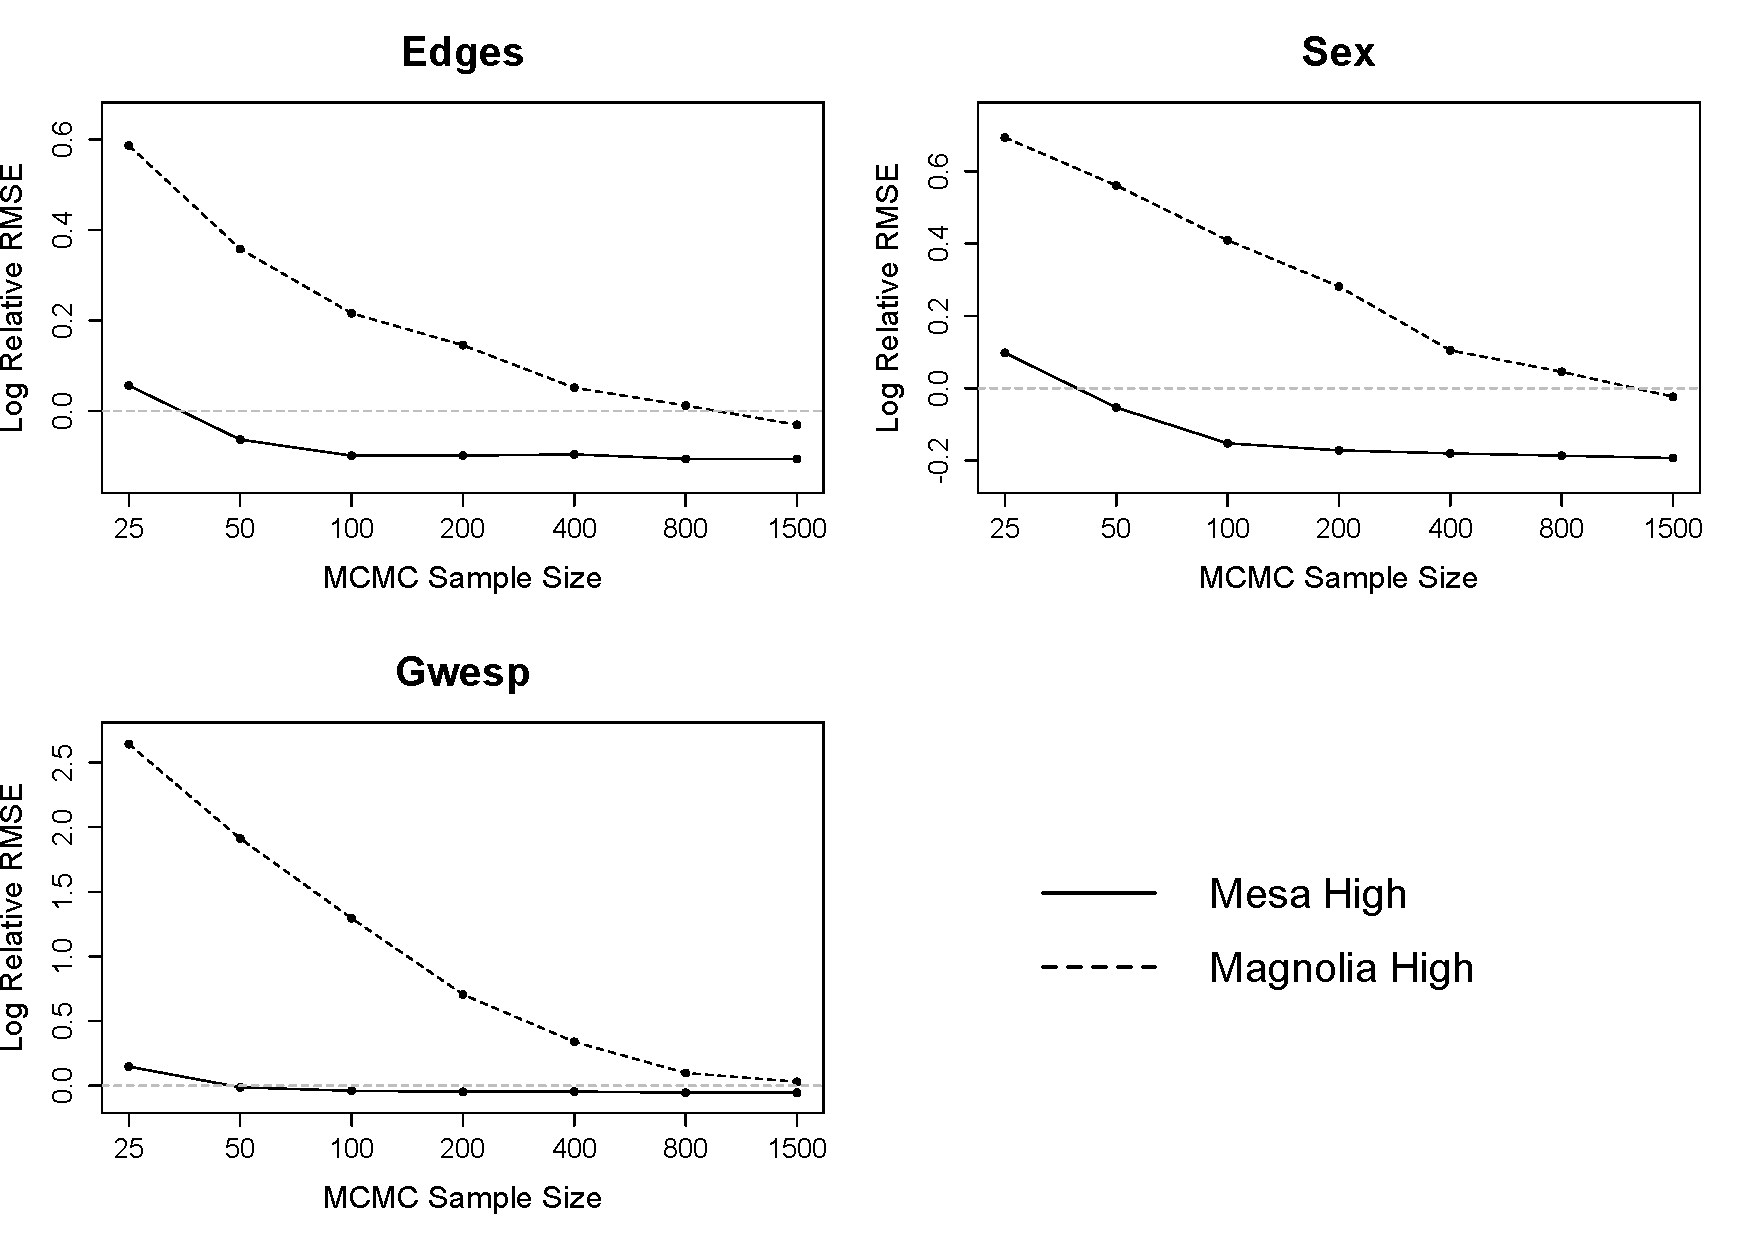
\includegraphics[scale=.5]{RMSE_paper}
\caption{The log of the ratio of the RMSE for the MCMLE to the MPLE for different sample sizes and two different networks, Faux Mesa High and Faux Magnolia High}
\label{rmse}
\end{center}
\end{figure}

\noindent The plots support the fact that larger networks require a larger sample size of simulated networks in order for the MCMLE to outperform the MPLE. While the fairly small Faux Mesa High network only requires a sample size of about 50 networks the larger Faux Magnolia High network already requires a sample size of at least 1500 networks for the MCMLE to surpass the MPLE. These results propose especially for very large networks (e.g. social media data) the question, of how large the sample size has to be set in order to justify the approximately exact, but computationally expensive MCMLE method. The identification of the required sample size is not only becoming more difficult as the size of the network increases, but an increase of the sample size will also extends the mere computation time. 


\section*{Bootstrapped MPLE}
As discussed in the previous section, the MPLE converges to the MLE as the size of the network increases. Moreover, the MPLE is able to outperform the MCMLE if the sample size is not chosen large enough. The main reason why the MCMLE is still widely preferred is that in contrast to the MPLE, it does not underestimate the variance of its estimates \cite{vanDuijnetal2009}. By the definition of the ERGM it is obvious that this model is an exponential family distribution where $\theta$ is the natural parameter and $\Gamma (Y)$ is the sufficient statistic. This allows us to work in the framework of exponential family distributions and as a consequence, leads to the conclusion that the sampling distribution of the MLE is multivariate normal with mean vector equal to the MLEs and a covariance matrix equal to the inverse of the negative Hessian matrix $[-H]^{-1}$ of the likelihood function at the MLE. The problem with the MPLE is that calculating $[-H]^{-1}$ by the pseudolikelihood function will underestimate the variance of the MPLE \cite{vanDuijnetal2009}, resulting in an underestimate of the width of the confidence intervals. van Duijn et al. show that constructing 95\% MPLE confidence intervals can result in intervals that only comprise the true value in less than 75\% instead of the demanded 95\%. In this paper, we are going to refer to the MPLE confidence intervals as \textit{logistic regression confidence intervals} simply because the MPLE is calculated using logistic regression methods that also use the inverse of the negative Hessian matrix as an estimate for the covariance matrix. \\[0.3cm]
\begin{figure}[h]
\begin{center}
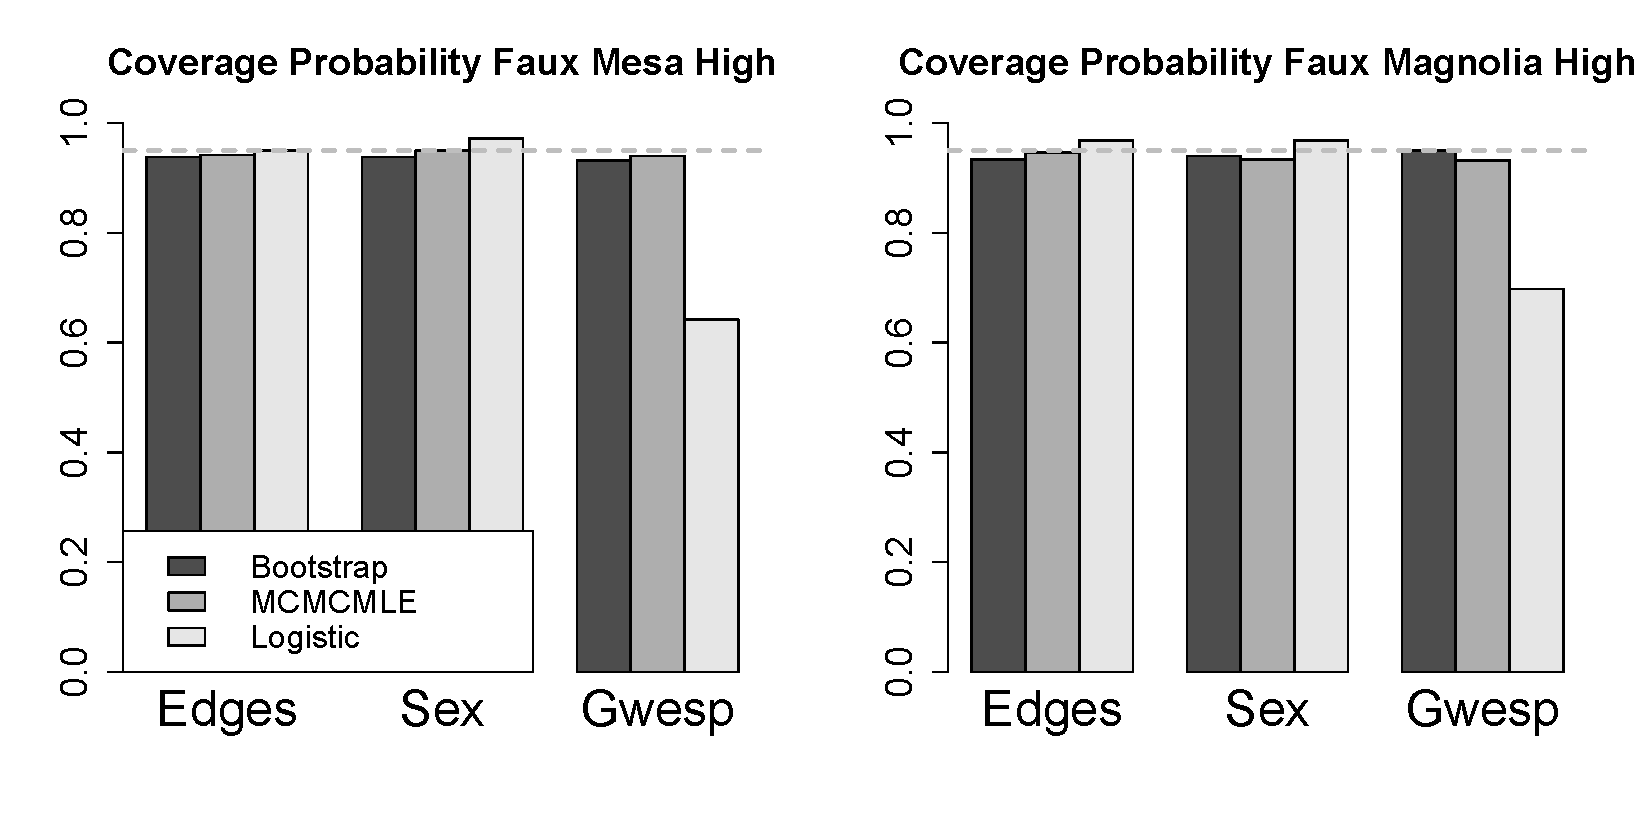
\includegraphics[scale=.5]{Coverage_Mesa_Magnolia_height05}
\caption{The Coverage Probability results of the Faux Mesa High network (left) and of the Faux Magnolia High network (right) for bootstrapped MPLE, MCMLE and logistic regression }
\label{coverage}
\end{center}
\end{figure}

\begin{figure}[H]
\begin{center}
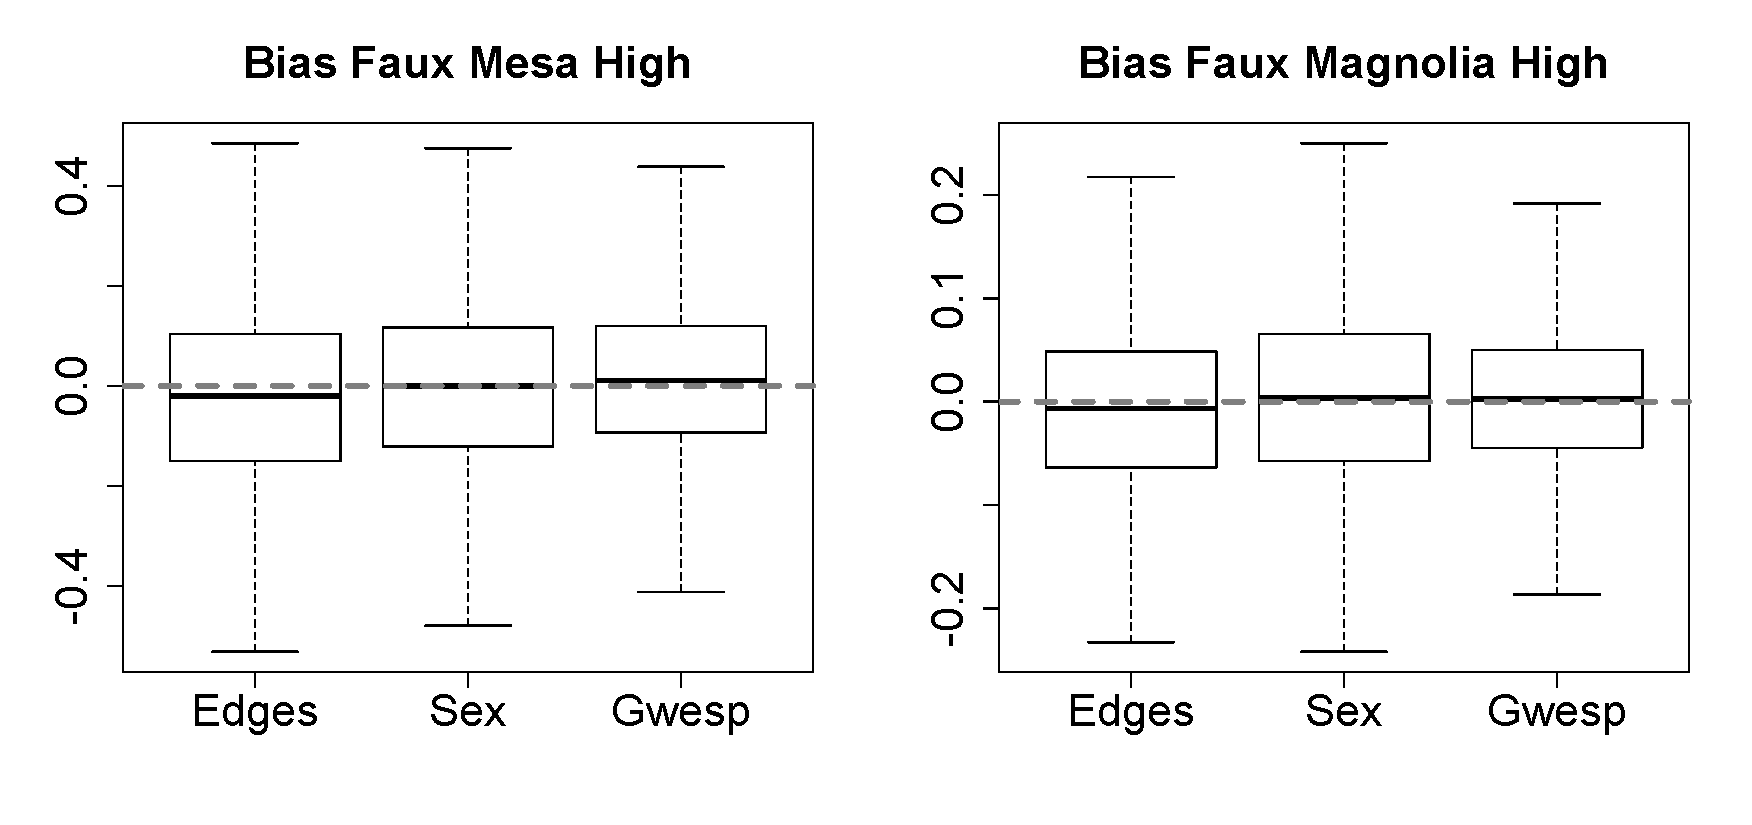
\includegraphics[scale=.40]{bias_plots_05}
\caption{The boxplots visualize the bias $(\hat{\theta}-\theta)$ over the 500 iterations for the Faux Mesa High network (left) and the Faux Magnolia High network (right).}
\label{bias}
\end{center}
\end{figure}
\noindent Since the MPLE has the advantage of being approximately exact and computationally inexpensive, but has the disadvantage of underestimating corresponding confidence intervals, we are going to apply a technique, referred to as \textit{bootstrapped MPLE}, that was first introduced by Desmarais and Cranmer \cite{Desmarais.2012} and provides a consistent estimate of MPLE confidence intervals. Desmarais and Cranmer argue that this bootstrapped MPLE is a multivariate \textit{M}-estimator \cite{Huber1981}, a special class of robust estimators, meaning that this algorithm consistently estimates the confidence intervals of the MPLE.



\noindent We verify the consistency of the bootstrapped MPLE by conducting a simulation study on the same two networks with the same paramtrization as in the previous chapter: The Faux Mesa High friendship network and the Faux Magnolia High friendship network. \\[0.3cm]
For the simulation study, we determine the MPLE for the model and treat these estimates as the networks' 'true' parameter values. We then use these parameter values to simulate a sample of $1000$ networks from the distribution of $Y$. For each of the $1000$ networks, we calculate 95\% confidence intervals based on the MCMLE and the logistic regression and examine whether the 'true' parameter values lie in these intervals. In addition, we determine the bootstrapped MPLE confidence intervals by sampling $500$ networks for each of the originally sampled $1000$ networks, by using the respective MPLE as parameter values. For every newly sampled network, we again determine the MPLE and then take the $2.5$th and $97.5$th percentile of the $500$ MPLE estimates to obtain a 95\% bootstrap confidence intervals. Similar as for the MCMLE and the logistic regression, we verify whether the 'true' parameter value can be found in the bootstrapped confidence interval. 



\noindent Figure \ref{coverage} visualizes the coverage percentages for each of the three methods for both networks. The dashed line is set at $0.95$ and represents the optimal value. It is in evidence that the bootstrapped MPLE performed equally well as the MCMLE, achieving results that obtain the true parameter values in approximately 95\% of the cases. Additionally, a difference in the results between the smaller Faux Mesa High network and larger Faux Magnolia High network is not identifiable. Similar to the results of van Duijn et al. \cite{vanDuijnetal2009} our results for the logistic regression differ distinctively from the anticipated 95\%, visualizing that the MPLE underestimates the variance of its estimates.
Figure \ref{bias} illustrates the bias between the 'true' network coefficients $\theta$ and the MPLE estimates. \textcolor{blue}{(=> not degenerate?, maybe provide boxplots for scnetwork)}
\noindent This simulation study shows that bootstrapped MPLE is able to overcome the main disadvantage of the MPLE by retaining the validity of confidence intervals. Furthermore, this method also adopts the advantage of the MPLE of being consistent. However, the main advantage of the bootstrapped MPLE is the rapidity of the estimation that provides a computational benefit, especially if the size of the examined network is extremely large.

\section*{Cosponsorship Network Data}

In order to demonstrate the computational advantage of the bootstrapped MPLE to the commonly used MCMLE we apply both approaches to the data on Cosponsorships in the U.S. Senate and U.S. House of Representatives for the 93rd to 108th Congresses developed by Fowler (2006) \cite{Fowler2006a} \cite{Fowler2006b}. The cosponsorship network consists of 2635 nodes and contains information of over 280,000 pieces of legislation proposed in the U.S. House and Senate for the time period 1973 - 2004. In this network each node indicates on cosponsor and an edge indicates the link of each cosponsor of a piece of legislation to its sponsor. The endogenous statistics we include into this model are the number of edges and the alternating k-star statistic as it was introduced by Snijders et al. \cite{SnijdersTomA.B..2006} and modified by Hunter and Handcock (2006) \cite{Hunter.2006}. The alternating k-star statistic adds one network statistic to the model equal to a weighted alternating sequence of k-star statistics with weight parameter $\lambda$ and is a way to include a networks entire degree distribution as a network statistic. In this model we fix the weight paramter $\lambda=0.4975$. 
Snijders et al. \cite{SnijdersTomA.B..2006} introduced an approach involving $k$-star statistics $S_1(A), \dots , S_{N-1}(A)$, where $S_k(A)$ denotes the number of $k$-stars in the network, $k \in \{1, \dots , N-1\}$. For simplicity, let us define
$$S_k(A):=\Gamma_{star(k)}(A) $$
\textit{define kstar}.
Note that in every network $S_1(A)=\Gamma_{edges}(A)$, i.e., $S_1(A)$ is equal to the number of edges in the network.
On this basis, Snijders introduces the \textit{alternating k-star statistics}
\begin{equation*}
\mathfrak{S}(A,\lambda):= \sum_{k=2}^{N-1}(-\cfrac{1}{\lambda})^{k-2}S_k(A)=    S_2(A)-\cfrac{S_3(A)}{\lambda}+ \dots + (-1)^{N-3}\cfrac{S_{N-1}(A)}{\lambda^{N-3}}
\end{equation*} 
Models with this statistic and a fixed decay parameter turn out to be standard ERGMs and Hunter and Handcock \cite{Hunter.2006} succeeded in proving that one can also rewrite alternating k-stars as a function of a network's degree distribution
\begin{equation}
\mathfrak{S}(A,\lambda)= \lambda\Biggr(\lambda\sum_{j=1}^{N-1}\Biggr( 1-\biggr(1-\cfrac{1}{\lambda}\biggl)^j\Biggl)D_j(A) + 2S_1(A)\Biggl)
\label{alto}
\end{equation}
where $D_j(A):= \Gamma_{deg(j)}(A)$ is the number of nodes with and degree of $j$. 
In the next step, we define the \textit{geometrically weighted degree} statistic as the first summand of (\ref{alto})
\begin{equation}
\Gamma_{gwd}(A,\lambda):= \lambda\sum_{j=1}^{N-1}\Biggr(1- \biggr(1-\cfrac{1}{\lambda}\biggl)^j\Biggl)D_j(A)
\end{equation}
At this point it also becomes obvious where the \textit{geometrically} comes from. It simply refers to the geometric sequence $(1-\frac{1}{\lambda})^j$ which appears in these statistics.\\[0.3cm]
\textbf{continue here}
The two nodal attributes we consider for this network are the year the majority opinion was drafted as well as an attribute that indicates whether a case appears on the Oxford list of salient cases. In order to include nodal covariates into the ERGM, the vector of nodal attributes is expanded into an artificial matrix $C$, which has the same dimensions as $G$. The first row of matrix $C$ consists of the first actor's attribute, repeated $N$ times. The second row of matrix $C$, consists of the second actor's attribute, repeated $N$ times, and so on. Then, the statistics for a nodal covariate is defined as
$$\Gamma_{nodal}: \mathcal{G}(N) \to \mathbb{R}~~,~~G \mapsto \sum_{i<j}^{N}g_{ij}c_{ij}$$
Beside these two nodal attributes, we furthermore include the difference between the years of publication as an edge attribute. An edge attribute can be written as a matrix $E$ of the same dimensions as the observed adjacency matrix $G$. In this case entry $e_{ij}$ is filled with the absolute difference between the year of case $i$ and case $j$. Then, the corresponding statistic can be calculated the same way as nodal covariates. Since we do expect a non-linear effect for this edge attribute, we include this variable as a second-degree polynomial by creating a matrix $E^2$, where the matrix gets squared component wise.\\[0.3cm]
We estimate the coefficient of this matrix using both techniques, the MCMLE and the bootstrapped MPLE. The MCMLE requires a sample size of at least $100000$ networks to converge. The bootstrapped MPLE was estimated by using 500 simulated networks. As we described in the chapter {\it Estimation}, only one edge at a time is changed when simulating networks. For better comparison, we chose the same Burn-In ($163840$ MH-steps) and the same number of iterations ($10240$ MH-steps) for sampling networks. The results can be found in table \ref{sc_results}.\\[0.3cm]


\begin{table}[]
\hspace*{-1.5cm}
\begin{tabular}{|
>{\columncolor[HTML]{EFEFEF}}l |l|l|l|l|l|l|}
\hline
\cellcolor[HTML]{EFEFEF}                   & \multicolumn{2}{c|}{\cellcolor[HTML]{EFEFEF}MCMLE}                   & \multicolumn{2}{c|}{\cellcolor[HTML]{EFEFEF}Logistic Regression}       & \multicolumn{2}{c|}{\cellcolor[HTML]{EFEFEF}bootstrapped MPLE}     \\ \cline{2-7} 
\multirow{-2}{*}{\cellcolor[HTML]{EFEFEF}} & \cellcolor[HTML]{EFEFEF}Estimate & \cellcolor[HTML]{EFEFEF}St. Error & \cellcolor[HTML]{EFEFEF}Estimate & \cellcolor[HTML]{EFEFEF}St. Error & \cellcolor[HTML]{EFEFEF}Lower Bound & \cellcolor[HTML]{EFEFEF}Upper Bound \\ \hline
Edges                                      & -5.657                           & 0.028                             & -4.568                       & 0.038                                    & -5.160 & -4.530  \\ \hline
Nodecov.Salience                           & 0.592                            & 0.012                             &   1.482                               & 0.009                                   & 1.413 & 1.890  \\ \hline
Nodecov.Year                               & 0.253                            & 0.012                             &     0.208                             & 0.015                                   & 0.182 & 0.504  \\ \hline
Absdiff.Year                               & -2.470                           & 0.160                             &  -3.121                                & 0.194                             & -3.308 & -2.434  \\ \hline
Absdiff.Year.Squared                       & 0.221                            & 0.066                             &   0.436                               & 0.080                                   & -0.028 & 0.517  \\ \hline
DSP(0)                                     & 0.0005                           & 0.0002                            &    0.021                              & 0.0002                                   & 0.019 & 0.031  \\ \hline
ESP(0)                                     & -3.129                           & 0.012                             &    -2.162                              & 0.004                                   & -2.179 & -1.511  \\ \hline
\end{tabular}
\caption{Estimation results for the Supreme Court Network using MCMLE, bootstrapped MPLE and logistic regression}
\label{sc_results}
\hspace*{-1cm}
\end{table}


\noindent The bootstrapped MPLE is not only simple and fast, it is also embarrassingly parallel, meaning that there is no problem separating the computation into several tasks. In other words, by using multiple cores, the computing time for estimating bootstrapped MPLE confidence intervals can be reduced substantially. Figure \ref{comptime} illustrates the relative computing time of the bootstrapped MPLE using 500 simulated networks and the MCMLE for the three networks Faux Mesa High (205 nodes), Faux Magnolia High (1461 nodes) and Supreme Court Citation (9223 nodes) for an increasing number of computing cores. For the small network we simulate $2000$ networks using a MCMC interval of $2000$ steps, for the medium network we simulate $8000$ networks using a MCMC interval of $5000$ steps and for the large network we simulate 1 million networks using $10,000$ MCMC steps in order to approximate the likelihood appropriately. The chosen sample sizes and MCMC steps are necessary to guarantee a good model fit. We define the simulation time of the bootstrapped MPLE as a function of the number of available computing cores x:
$$\text{boostrapped MPLE time} = \text{network simulation time} + \cfrac{500 \cdot \text{MPLE estimation time}}{x}$$     
Based on this, we define the relative computing time as
$$\text{relative computing time}= \cfrac{\text{bootstrapped MPLE time}}{\text{MCMLE time}}$$
This means that a relative computing time greater than 1 indicates that the MCMLE computing time is shorter, while a relative computing time smaller than 1 indicates that the bootstrapped MPLE provides faster results. 
\begin{figure}
\begin{center}
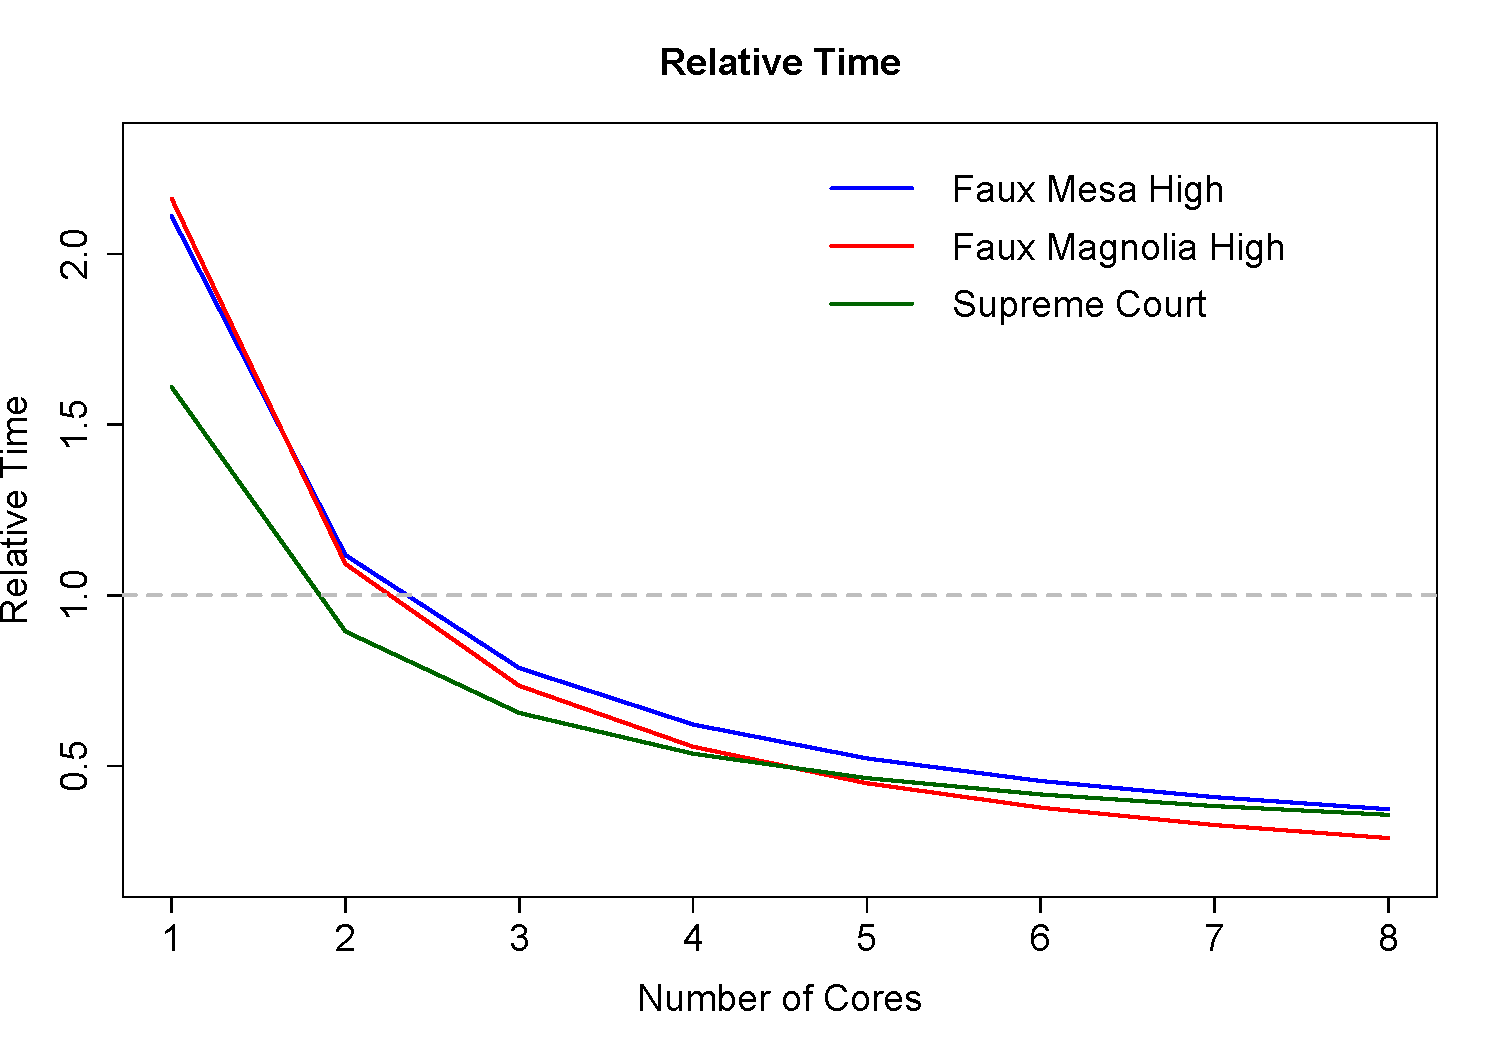
\includegraphics[scale=.45]{rel_time}
\caption{The y-axis gives the ratio of the bootstrapped MPLE time to that of the MCMLE time. Values below 1 indicate that the bootstrapped MPLE requires a shorter computing time.}
\label{comptime}
\end{center}
\end{figure}
Figure \ref{comptime} demonstrates that the two high school friendship networks only require three cores for the bootstrapped MPLE to outperform the MCMLE. Even more interesting is that the even larger Supreme Court Citation network only requires two cores for the bootstrapped MPLE to outperform the MCMLE.\\[0.3cm]
One of the major disadvantages of MPLE over MCMLE is that it cannot assess {\it degeneracy}. When fitting an ERGM one usually has to deal with the problem of unreliable approximatively likelihood estimates for the model's parameters. The reason why degeneracy occurs is that the stochastic process generated by the MCMC-algorithm does not necessarily hold through the model's defined distribution of the random variable $Y$ as stationary distribution (see Handcock \cite{Handcock.2003} and Rinaldo et al. \cite{Rinaldo2009}). The bootstrapped MPLE, however, allows assessing degenerate models as well. In order to verify whether a model is degenerate or not, one can take a look at density and trace plots as visualized in figure ??. The trace plots on the left side depict the the attained values via MCMC simulated networks for every single statistic included into the model, centered on the statistic values of the observed network. The plots on the right side visualize the empirical density function of the respective statistic, based on the simulated networks (Hunter and Handcock \cite{Hunter.2006}). For a non-degenerated model the empirical density function should be symmetrical around zero for every included centered statistic, since this corresponds with the expected value of a centered statistic (compare equation (\ref{assumption})). 
Otherwise, the values of the simulated networks systematically differ from the corresponding statistics in the observed network, making it unreasonable to assume that the simulated networks originate from the same distribution as the observed network. Furthermore, the trajectories in the trace plot should not indicate a dependence structure. This would be a signal that the constructed stochastic process violates the Markov properties.
$$\text{insert density plots and trace plots}$$

\begin{itemize}

\item describe advantage over MPLE (better coverage) and MCMLE (faster)
\item can easily be parallelized/ using multiple cores -> increases speed
\item this method is also able to detect degeneracy
\item include table with boot MPLE results and MCMLE results
\end{itemize}


 \section*{Other chapters}
 
 \begin{enumerate}
 \item Fields that made fruitful use of the MPLE for networks, e.g. Boltzmann machine
 \item Examples where a logit approach was used instead of an ERGM, because the network was too big and it was too time consuming using the MCMLE. We can then try to apply the bootstrapped MPLE approach.
\end{enumerate}   
   


 \section*{Results/Discussion}
\begin{itemize}
  
 \item  Bootstrap MPLE is an improvement of the MPLE and performs just as good as the MCMLE. \\
\item Bootstrap MPLE has the advantage of being fast + multiple cores\\ 
\item Bootstrap MPLE is consistent\\
\item Conclusion: For very large networks the Bootstrap MPLE approach is more reasonable
   
\end{itemize}

   
\newpage


\bibliography{bib} 
\bibliographystyle{plain}


\end{document}
